
\section{Experiments}\label{sec:exp}
To evaluate the effectiveness of our approach, we conduct a series of comparison experiments and ablation studies on two widely used datasets,~\emph{i.e.,} YouTubeVOS \cite{xu2018Youtube} and DAVIS \cite{davis_2017}, under different settings.
%We test on two datasets, YouTubeVOS \cite{xu2018youtube} and DAVIS \cite{davis_2017}, to compare the proposed STSENet with state-of-the-art methods. %Several ablation studies are conducted to prove the effectiveness of spatial details and temporal information in video inpainting.



\begin{table*}[t]
	\caption{Comparisons with six state-of-the-art methods on YouTubeVOS. Our method outperforms all other methods on three video quality metrics, with comparable temporal smoothness and fast inference speed.}\smallskip
	
	\centering
	\resizebox{2.0\columnwidth}{!}{
		\smallskip\begin{tabular}{c|c|c|c|c|c|c|c|c|c|c|c|c|c }
			\hline
			&\multicolumn{4}{c|}{Fixed Square Mask}& \multicolumn{4}{c|}{Moving Square Mask}&\multicolumn{4}{c|}{Free-Form Mask}  & Inference \\
			\cline{2-13} 
			&PSNR & SSIM & FID &Tem-ERR & PSNR & SSIM & FID  &Tem-ERR & PSNR & SSIM & FID  &Tem-ERR &Speed (fps)\\
			\hline
			Edge-Connect \cite{nazeri2019edgeconnect} &28.6446 &0.9484  &   38.2116  & 0.02403 &   
			30.7478 & 0.9647 &  16.2739  & 0.02807 &
			25.6693  & 0.9088 &  43.0366 & 0.04130  &22.81 \\
			\hline
			CombCN \cite{wang2019video} &27.9668 & \underline{0.9515} &  40.7199  &   0.02252 &  
			31.5776    & 0.9678 &  13.8383& 0.02443 &  
			32.1862 & 0.9626 & 19.1191 & 0.03241&8.1634 \\
			\hline
			
			
			DVI \cite{Kim_2019_CVPR1}& 28.0846&0.9468 &  39.9377  & \textbf{0.01817} & 
			36.8598    & 0.9728 &7.2315  &\textbf{0.01946} &
			\underline{33.5549}    & \underline{0.9646} & \underline{9.3797} & \textbf{0.02188} &1.2275  \\
			\hline
			DFVI \cite{Xu_2019_CVPR} &29.0531 & 0.9497 &  \underline{32.8860} & \underline{0.02025} & 
			\underline{37.8241}& \underline{0.9772} &\underline{6.3746}  & \underline{0.02258} &
			32.6287 &0.9618  &  11.1501 & 0.02358  &0.5620 \\
			\hline
			
			Copy-and-Paste \cite{lee2019copy}&
			27.8722 &   0.9040 &  35.5054 & 0.02282 &
			
			33.0092 &  0.9388 &  10.5099 & 0.02500 & 
			
			30.2559 & 0.9106 & 31.3721 & 0.02968 
			& 1.4741
			\\
			
			\hline
			
			
			OPN \cite{oh2019onion} & \underline{29.2663} &0.9149 & 37.9550 &0.02328 &
			
			33.3254 & 0.9381  & 12.1887 &0.02498 &
			
			31.7570  & 0.9211 & 24.0585 
			&0.02782 &
			3.8239 \\
			
			
			\hline
			
			
			
			Ours &\textbf{30.0590} &\textbf{0.9543}&   \textbf{27.2431} & 0.02082 &
			\textbf{38.8186} & \textbf{0.9824} & \textbf{2.3455} & 0.02388 &
			\textbf{35.9613}  & \textbf{0.9721}&  \textbf{ 5.8694}  & \underline{0.02278}  &5.1546\\
			
			\hline
		\end{tabular}
	}
	\label{tab:sem}
\end{table*}


\subsection{Experimental Settings}
\noindent \textbf{Mask Setting.} Considering different real-world applications, we test four kinds of mask settings in this paper, which are different in shapes and positions of the missing regions. 
%The first and the second settings aims to recover rectangular regions, which are common in watermark removal.
\begin{enumerate}
\item Fixed square mask: The size and position of the missing square regions are fixed through the whole video. 
\item Moving square mask: The position and size of the square masks change over frames. 
\item Free-from mask: We apply irregular masks which imitate hand-drawn masks on each frame, following \cite{liu2018partialinpainting}. 
\item Foreground object mask: This type of mask is defined to line out foreground objects in videos and used for testing object removal.
\end{enumerate}

\noindent\textbf{Dataset.} 
YouTubeVOS and DAVIS are widely used for evaluating video inpainting results in recent studies.
YouTubeVOS consists of 4,453 video clips that contain more than 70 categories of common objects. 
The videos are split into three parts, 3,471 for training, 474 for validation, and 508 for testing. Since YoutubeVOS has no dense foreground mask annotations, we only use it for evaluation under mask settings (1), (2), and (3). 
% 
DAVIS dataset contains 90 video sequences that are annotated with foreground object masks for testing and 60 unlabeled videos for training.






\begin{figure*}[tb]	
\centering	
	\includegraphics[width=\textwidth]{viszong} % Reduce the figure size so that it is slightly narrower than the column. 	Don't use precise values for figure width.This setup will avoid overfull boxes. 
	\caption{Comparison with state-of-the-art methods on the YouTubeVOS dataset under different mask settings. Our method 	produces results with more complete object structures and finer details.}	
\label{viszong}
\end{figure*}



\noindent \textbf{Implementation details.} 
All the models are tested on a TITAN X (Pascal) GPU with frame size $256 \times 256$.
For training data, we randomly sample a training clip every 40 frames from each video in the dataset. Our training process consists of three steps. First, we train ENet with learning rate set as $1e-4$ for $G^E$ and $1e-5$ for $D^E$. 
Then we train TexNet while fixing ENet. The learning rate is set as $1e-4$ for $G^T$, and $4e-4$ for $D^T$.
We first train ENet and TexNet without flow-constrained losses, and then add the flow losses to finetune the networks.
%ensemble module is finally trained while fixing all the other modules. Learning rate is $1e-4$.
An Adam optimizer with $\beta=(0.9, 0.999)$ is used for all sub-network training.
%We do not use weight decay.
As for the hyper-parameters, we set $\lambda_1=10.0,\lambda_2=0.2$, which will be analysed later. 
%, \lambda_3=0.1$.
{\color{blue} The detailed network architectures of ENet and TexNet are listed in the supplementary material.
During inference, we sequentially feed frames into the network. The network takes 5 frames as input and output the reconstructed frame $\widetilde{V}_t$ in one forward pass.
}

\noindent \textbf{Evaluation Metrics.} 
Different data preparations and evaluation metrics are used according to mask settings. We randomly generate masks for training videos in terms of mask settings (1), (2), and (3). 
Masked videos are used for testing.
Four commonly-used metrics, including structural similarity index (SSIM) \cite{wang2004image}, peak signal-to-noise ratio (PSNR), Fr{\'e}chet Inception Distance (FID) \cite{heusel2017gans}, and temporal warping error (Tem-ERR) \cite{Kim_2019_CVPR} are used to quantitatively evaluate the performance of our method. 
{\color{blue}Specifically, PSNR, SSIM, and FID focus on frame generation quality, while Tem-ERR is to assess the temporal smoothness.} 
For each training video at mask setting (4), we randomly select a test video from the 90 test videos in the DAVIS dataset and apply its masks for the current training video with random rotation, scaling, and translation.
Our inpainting network is first trained on the YoutubeVOS dataset and then finetuned on the DAVIS dataset. 
Since there are no ground truth video for mask setting (4) of foreground object removal, it is infeasible to do quantitative evaluations to measure the output quality. Instead, a user study is conducted.  



\subsection{Evaluation of Video Inpainting on YouTubeVOS}
We compare the proposed method with six state-of-the-art video inpainting methods \cite{nazeri2019edgeconnect,wang2019video,Kim_2019_CVPR1,Xu_2019_CVPR,lee2019copy,oh2019onion}
for the first three mask settings on the YouTubeVOS dataset.
%
We train \cite{nazeri2019edgeconnect,Xu_2019_CVPR} using their published codes and re-implement \cite{wang2019video} according to their paper. As for \cite{Kim_2019_CVPR1,lee2019copy,oh2019onion}, we use the officially provided model.


The quantitative results and inference speeds are reported in Table~\ref{tab:sem}.
It can be seen that our method outperforms state-of-the-art methods on most of metrics of generation quality.
First, in terms of three metrics of PSNR, SSIM, and FID about frame quality, our method outperforms all other methods, which demonstrates the effectiveness of introducing structure guidance into video inpainting.
Especially, compared with the 2D image inpainting method Edge-Connect~\cite{nazeri2019edgeconnect}, which also predicts edges to represent the target structure, our method greatly increases the completion performance by leveraging neighboring frames to complete edges and synthesize textures. 
Compared with other flow-based video inpainting methods without edge enhancement, our method shows great superiority, which can generate more temporally coherent and realistic contents. 

{\color{blue}
Second, in terms of Tem-ERR about temporal smoothness, our method outperforms most of existing methods, which proves that the temporal consistency constraint can exactly facilitate texture smoothness.
Specifically, in Table~\ref{tab:sem}, our method is comparable with DFVI and worse than DVI.
The reason is that DVI uses a recurrent feedback loop and a memory layer (LSTM) for temporal consistency, which has a strong ability of modeling temporal dependency. DFVI iteratively propagates pixels using optical flow. Both DFVI and DVI focuses on designing temporal modules to obtain smooth inpainting, thereby obtaining more smoothing results but much slower inference speed than our method. More importantly, under edge guidance, our method generates results with fine structural details, which obtains obviously higher generation quality (PSNR, SSIM, FID) than DFVI and DVI.
}

Third, our method is also very efficient, e.g., four times faster than DVI \cite{Kim_2019_CVPR1} and nine times faster than DFVI \cite{Xu_2019_CVPR}. 
The inference speed of Edge-Connect is faster than our method since it does not consider axillary temporal information between frames. 
%This result shows that our ENet and temporal consistency constraints are efficient and effective. 



{\color{blue} Besides, OPN \cite{oh2019onion} and Copy-and-Paste \cite{lee2019copy} are two recent methods that leverage non-local correlation between reference and target frames.
However, they only consider texture interaction between video frames, while ignoring the important edge-texture correlation.
Thus, the generation quality of our method is superior to that of both two methods with higher inference speed. It shows that the structure information introduced by edge guidance is important in video inpainting, and our method is capable of exploiting the correlation between video contents and object structures. }
%
%% Time performance analysis 

Finally, some inpainting examples are shown in Fig.~\ref{viszong}.
Compared with existing methods, the inpainting results predicted by our method are more realistic with finer details. 
We can observe that the frames completed using our method contain sharper object boundaries. This is achieved by the effectiveness of structure information in video inpainting.
%
It can also be seen that our method produces temporally smooth results when observing neighboring frames. More comparisons can be found in the supplementary video. 
%\cxj{show results?}

In summary, Both the quantitative and qualitative results demonstrate that our method is not a naive extension to utilize structure information in video inpainting.
The well-designed network architecture fully exploits structural guidance in video inpainting and brings large performance gain.





\begin{figure}[!t]
	\centering
	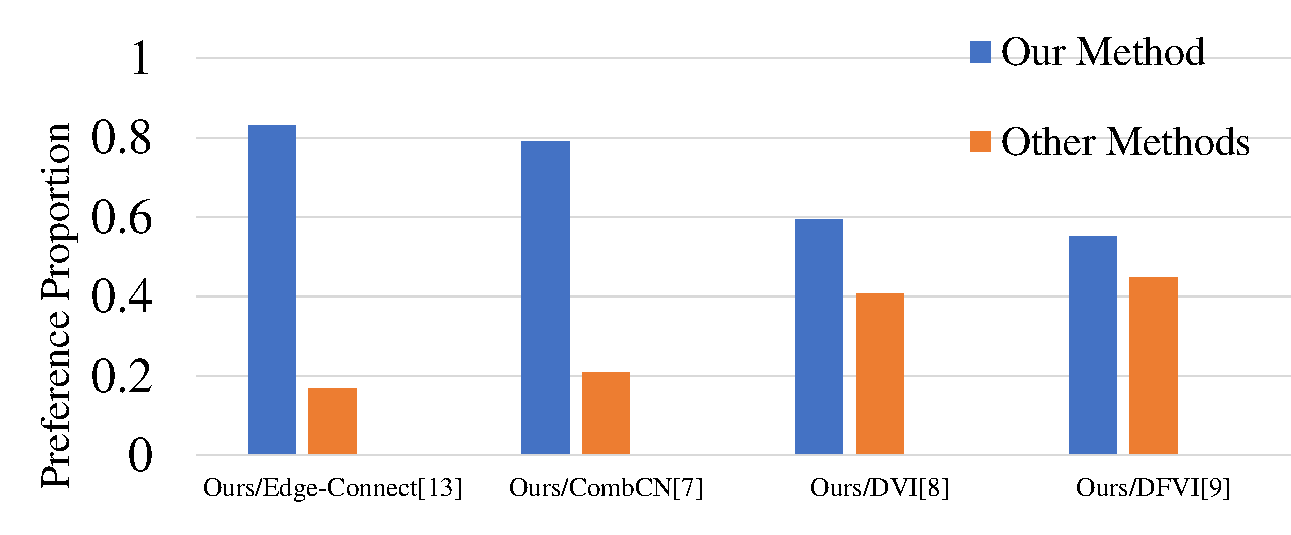
\includegraphics[width=1.0\columnwidth]{userstudy} % Reduce the figure size so that it is slightly narrower than the column. Don't use precise values for figure width.This setup will avoid overfull boxes. 
	\caption{Results of user study. The restored videos using our method are preferred by more participants compared with other state-of-the-art methods. }
	\label{userstudy}
\end{figure}






\begin{figure}[!t]
	\centering
	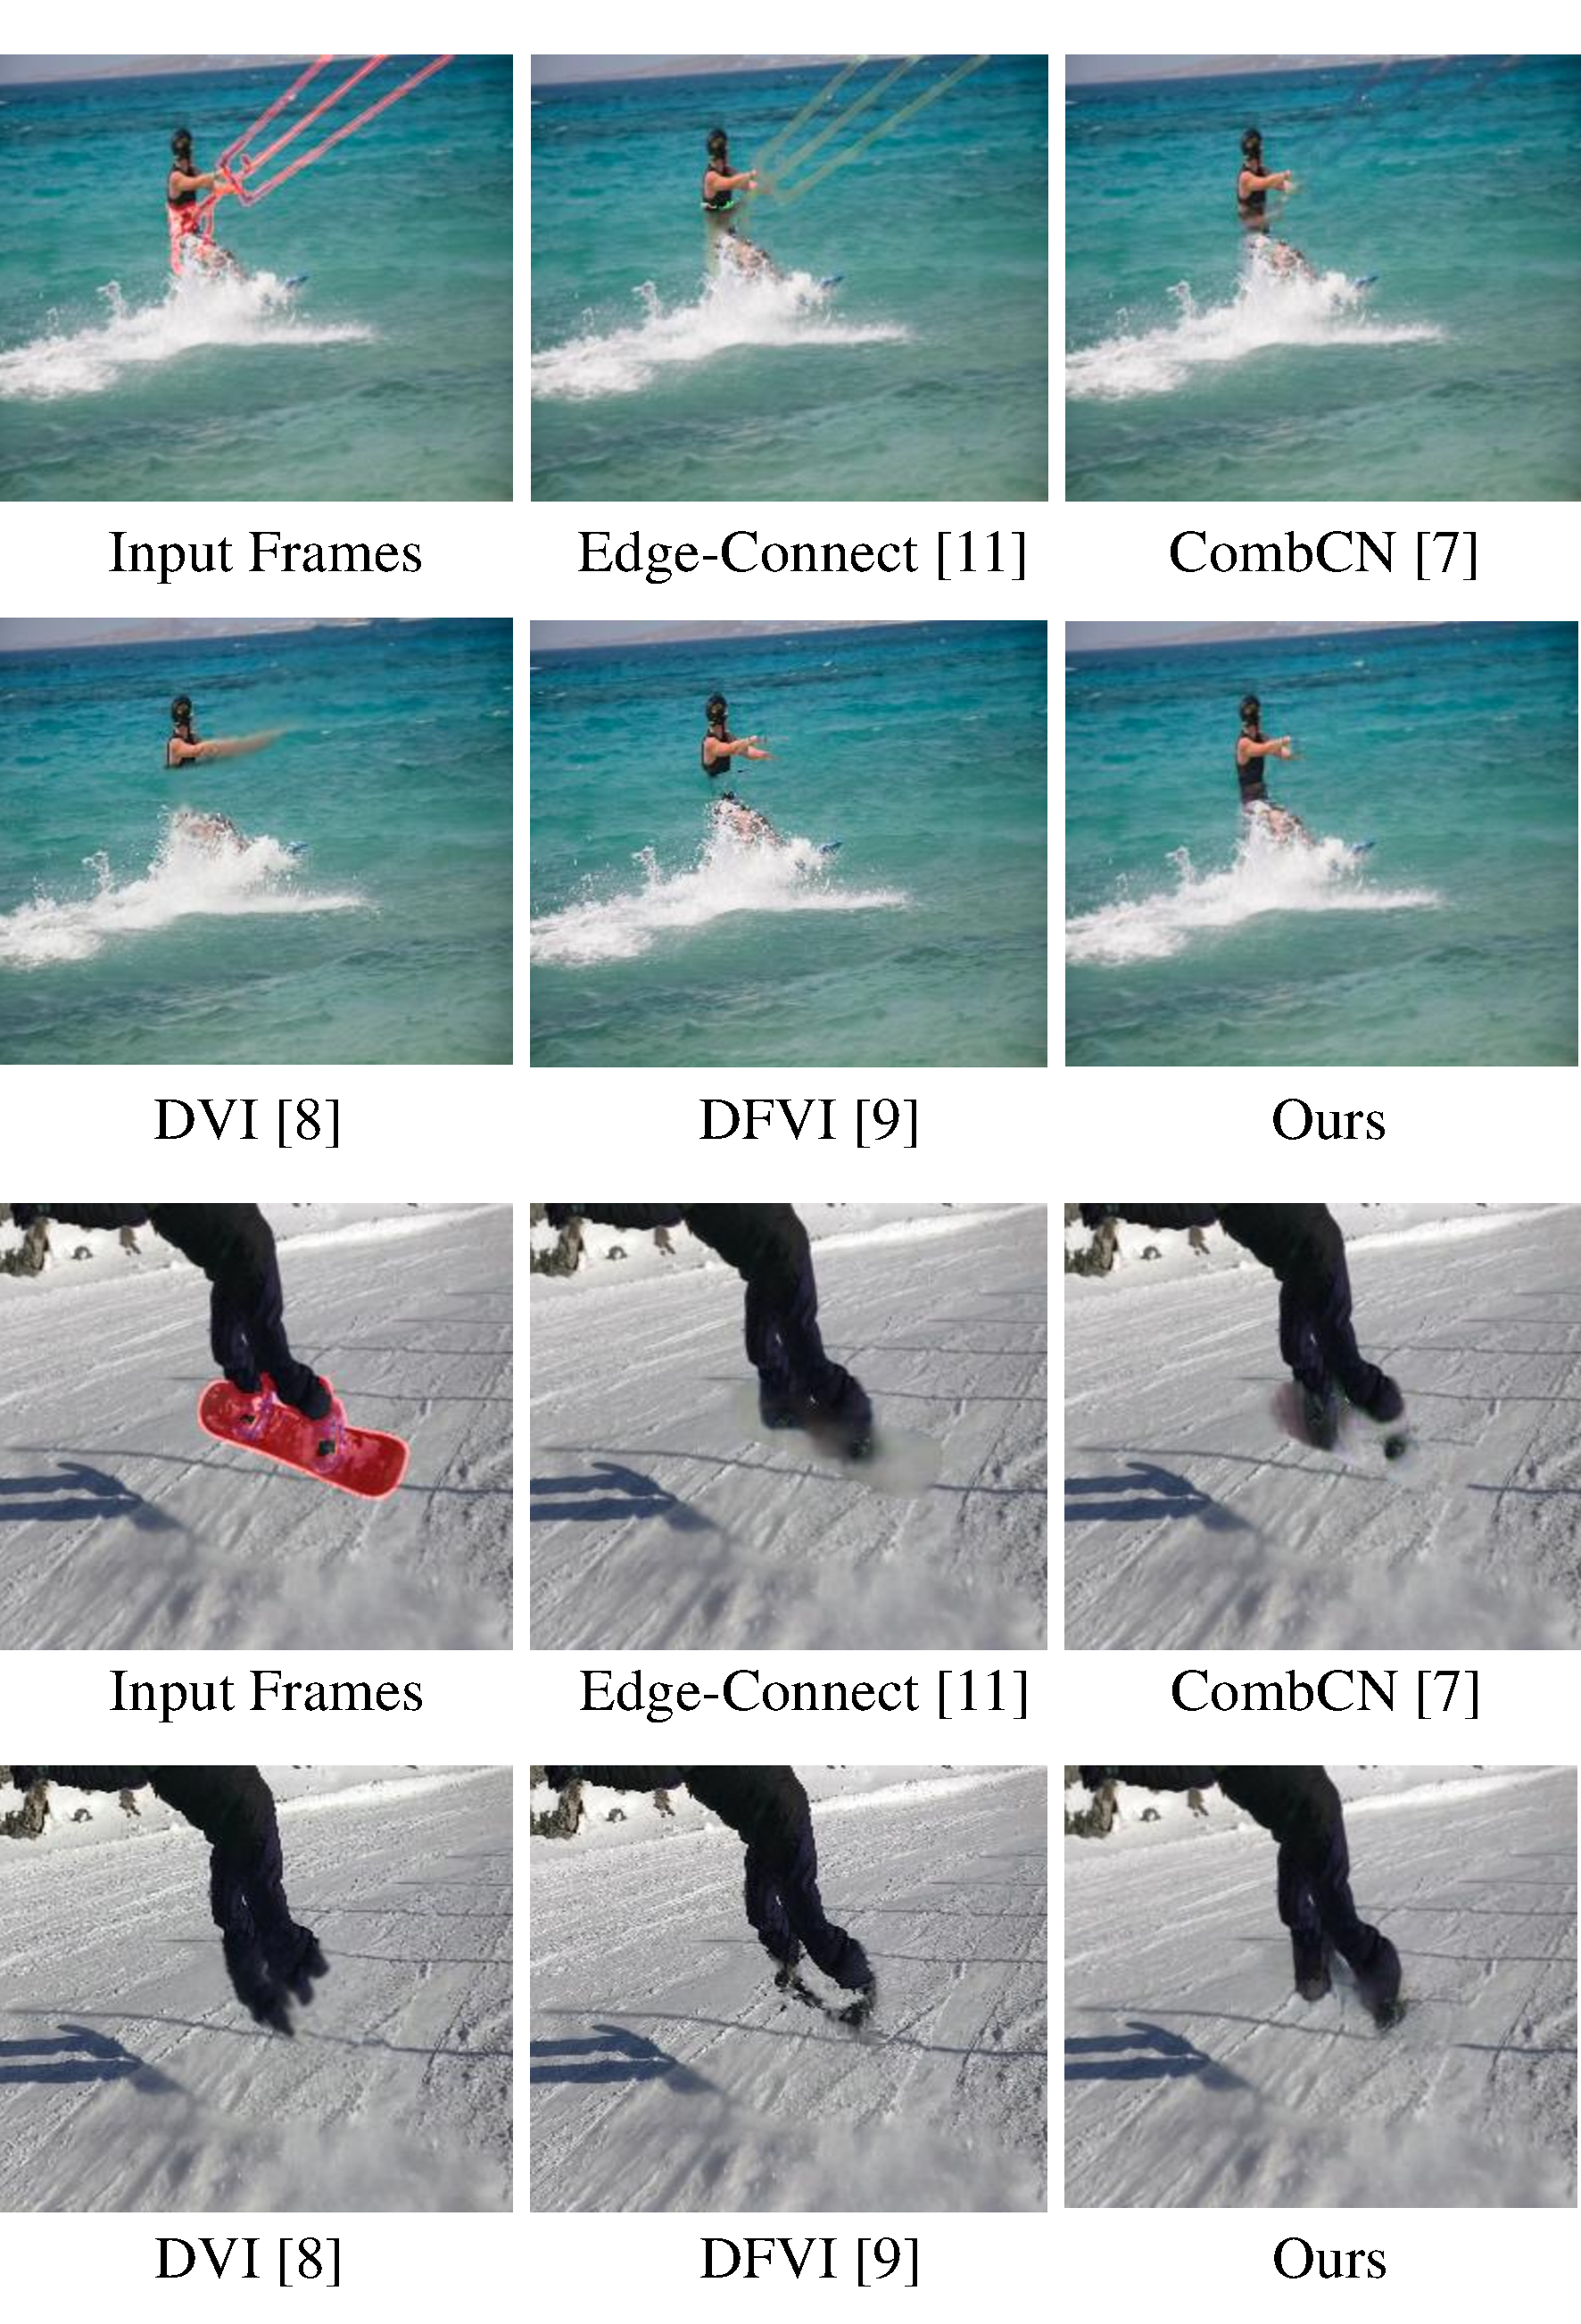
\includegraphics[width=0.85\columnwidth]{vis_forg} % Reduce the figure size so that it is slightly narrower than the column. Don't use precise values for figure width. This setup will avoid overfull boxes. 
	\caption{Results of object foreground removal. The red masks in input frames indicate the objects to be removed. Our method produces results with plausible structures and details.}
	\label{vis_forg}
\end{figure}

\subsection{Object Removal on DAVIS}


In regard to the foreground object mask setting that aims to remove undesired objects in videos, there is no ground truth for quantitative evaluation. 
Therefore, we conduct a user study on the DAVIS dataset to evaluate the visual quality of our method, compared with the four methods \cite{nazeri2019edgeconnect,wang2019video,Kim_2019_CVPR1,Xu_2019_CVPR}.
%
In each test, we show three videos to the subject at the same time. The original video with red masks indicating objects to remove is shown in the middle, while the inpainting results of our method and one of the other four methods are shown on the two sides in random order.
%  
The subjects can watch the videos repeatedly to better evaluate the differences.
For each video triplet, the subject is asked to choose which inpainting video is preferred.
44 subjects participated in our user study. 
Each participant watched averagely 20 triplets. 
Therefore, each pair of methods is compared about 220 times.
%Each method is compared about 200 times.

%


\begin{table*}[!t]
	\caption{Ablation studies on YouTubeVOS. Structure inference, structure attention model, and flow constrained loss are demonstrated effective in video inpainting.}\smallskip
	
	\centering
	\resizebox{2.0\columnwidth}{!}{
		\smallskip\begin{tabular}{c|c|c|c|c|c|c|c|c|c|c|c|c|c|c|c }
			\hline
			&\multicolumn{4}{c|}{Fixed Square Mask}& \multicolumn{4}{c|}{Moving Square Mask}&\multicolumn{4}{c|}{Free-Form Mask} & \#Params & GFLOPs &Inference \\
			\cline{2-13 } 
			&PSNR & SSIM & FID & TEM-ERR & PSNR & SSIM & FID & TEM-ERR & PSNR & SSIM & FID & TEM-ERR & (M)& &Speed (fps)\\
			
			\hline
			
			
			TexNet &28.0174 &0.9494  &  42.7164 &   0.02301 &    
			33.8131 &  0.9705  &8.2390  & 0.02713 & 
			30.0680& 0.9390 & 20.6358   & 0.02814  &  28.85& 476.5 &
			7.6335
			\\
			\hline
			+Edge  &29.5242 &  0.9520& 36.2097  & 0.02412 &    
			37.6630    & 0.9798 &3.5161   & 0.02579 &    
			33.8206    &0.9659  &    6.6651 & 0.02532 &42.26 & 849.7  &
			 5.2356 \\
			\hline
			
			+SAM &29.9918 &  0.9533 &  27.4198  & 0.02301 &   
			38.2433    & 0.9807 &   2.5083  &   0.02535 & 
			35.7783    &0.9712  &   5.8786 & 0.02517  & 42.33 &  859.7  &
			5.1546\\
			\hline
			
			
			
			
			+Flow &\textbf{30.0590} &\textbf{0.9543}&   \textbf{27.2431}  &\textbf{ 0.02082}  &
			\textbf{38.8186} & \textbf{0.9824} & \textbf{2.3455} &  \textbf{0.02388} &
			\textbf{35.9613}  & \textbf{0.9721}&  \textbf{ 5.8694} &  \textbf{0.02278}  &42.33 &  859.7 &
			5.1546\\
			
			\hline
			
			
		\end{tabular}
	}
	\label{tab:abl}
\end{table*}

The preference results in the user study are shown in Fig.~\ref{userstudy}. 
Comparing to Edge-Connect \cite{nazeri2019edgeconnect}, CombCN \cite{wang2019video}, DVI \cite{Kim_2019_CVPR1}, our results are preferred by a significantly larger portion of subjects.
%
When comparing with the flow-guided method DFVI~\cite{Xu_2019_CVPR}, our method is preferred by $55.24\%$ of the tests. 
Notably, our method is much faster than DFVI.
%
Fig.~\ref{vis_forg} shows two examples of object removal using different methods. 
We can see that the inpainted results generated by our methods are visually better than existing methods.
Compared to the blurry contents in the results of Edge-Connect, CombCN, and DVI, our method produces sharp object boundaries and fine visual details. Notably, though the completed contents using DFVI have sharp edges, the global structure of the human bodies is corrupted. In comparison, our method achieves more intact and plausible structure with fine details.
The results demonstrate the importance of utilizing structure information in video inpainting. 




\subsection{Ablation Study}
To demonstrate the effectiveness of each component in our network, we conduct a series of ablation studies on the YouTubeVOS dataset with the first three mask settings. 
%
We test four variants of our model. 
The baseline model `TexNet' only consists of the coarse-to-fine texture inpainting network without using edge maps as input and no SAM in the refinement module.
This model simply integrates neighboring frames to predict the missing content for the current frame.
%
Then we add the edge inpainting network ENet and feed the texture inpainting network with the completed edge maps to get the second model `+Edge'.
The third model `+SAM' is constructed by adding the structure attention module on the second model. 
Finally, we add the flow constrained loss during training to get our full model `+Flow'. Especially, we only add the flow constraints in the training stage, which means it brings no computation costs to the inference process.
The quantitative results are reported as in Table~\ref{tab:abl}. 

%

\subsubsection{Effect of Structure Clues}


\begin{figure}[t]
	\centering
	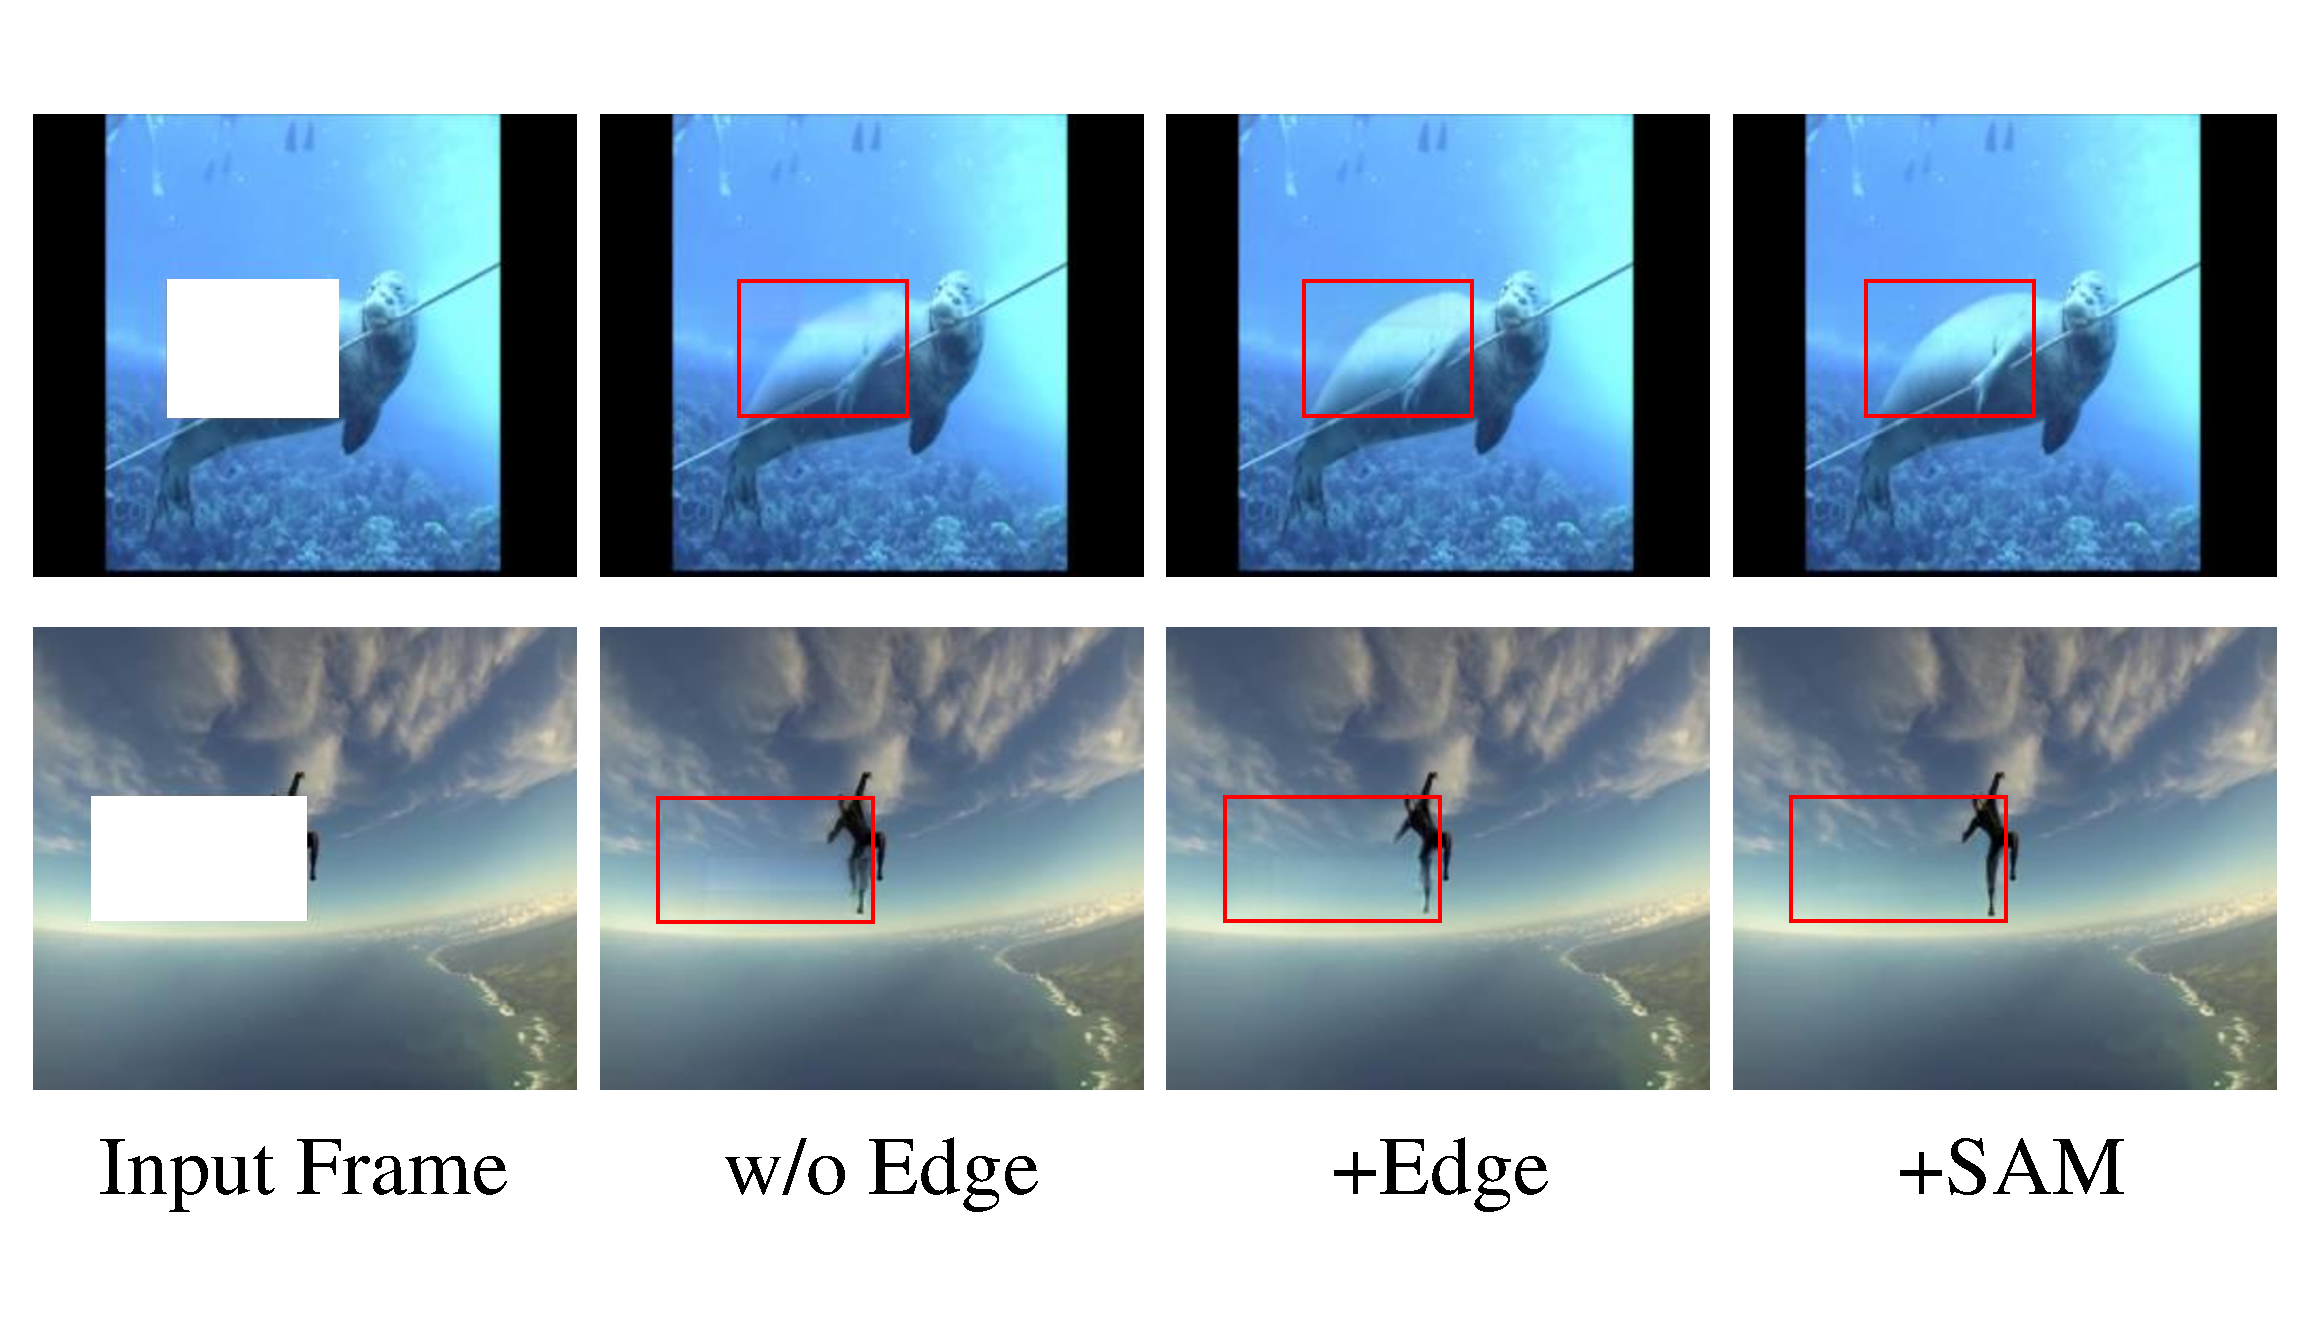
\includegraphics[width=0.97\columnwidth]{edgevis} % Reduce the figure size so that it is slightly narrower than the column. Don't use precise values for figure width.This setup will avoid overfull boxes. 
	\caption{Effects of structural guidance. By hallucinating edge maps first and then filling texture, we generate more completed and plausible target structure. Clearer boundaries can be obtained using the structure attention module.}
	\label{edgevis}
\end{figure}



In Table~\ref{tab:abl}, The model `+Edge' brings large improvement over the baseline model.
It indicates that sparse edges can provide effective structural guidance in video inpainting.
When we further add SAM, extra improvement is obtained, demonstrating that the spatial correlation between edges and textures can be better embedded and absorbed by the texture inpainting network than simply feeding the hallucinated edge maps as extra channels into TexNet. {\color{blue}Besides, the SAM does not bring too much cost to the whole network, according to \#Params and GFLOPs. The reason is that the inputs to SAM are down-sampled edge and video feature maps, of which the resolution is tolerant. Thus, the inference speed also shows that SAM is not a burden to the network. This proves that, in current setting, SAM can bring performance gains with tolerant cost and can be used in practice. However, when coming to high-resolution inpainting, SAM may put a high demand on computational resource.}
The above analysis proves that the edge clues are effective guidance in video inpainting, which helps the network to predict more plausible frames with completed and detailed structure.
Indeed, the structure inference module ENet brings extra time cost to the baseline TexNet from 7.6335 \emph{fps} to 5.2356 \emph{fps}.
This is deserved because the inpainting quality is significantly improved.

Fig.~\ref{edgevis} shows the results generated using the three variants. 
It is obvious that after introducing structural guidance, the inpainted frames become more visually pleasing with sharper object boundaries. 
Besides, the edge maps predicted by our method are reasonable and clear, which well represent the image structure and show the strong edge inpainting ability of ENet. 
Thus, it is crucial to explore structural details in video inpainting.
 



%\begin{figure}[t]	
%    \centering
%    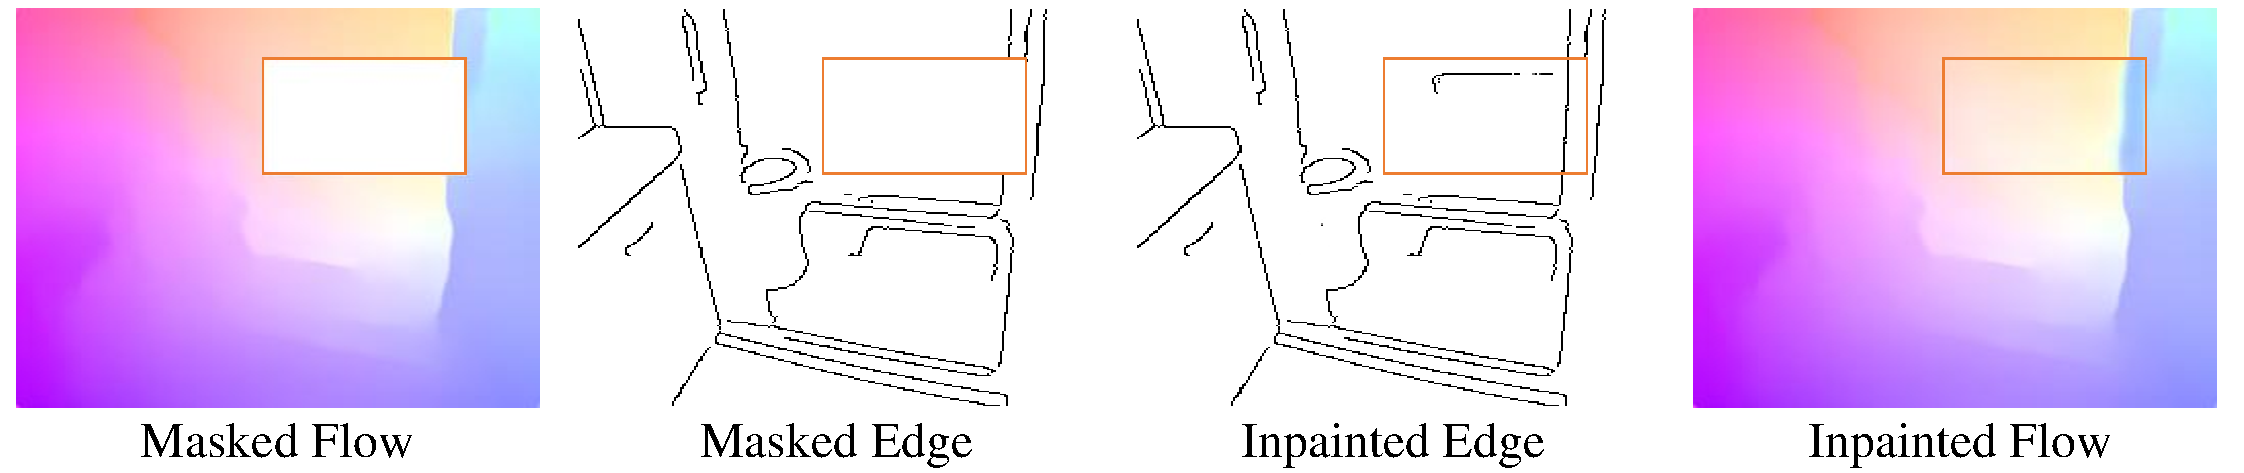
\includegraphics[width=1.0\columnwidth]{flowvis} % Reduce the figure size so that it is slightly narrower than the column. Don't use precise values for figure width.This setup will avoid overfull boxes. 
%    \caption{Visualized optical flow predicted by our method.}
%    \label{flowvis}
%\end{figure}


\begin{table}[t]
	\caption{Comparison of proposed structure attention module (SAM) and variants of attention modules on YouTubeVOS. SimAtt denotes a simple 2-layer spatial attention. SelfATT denotes the self attention module. SAM is capable of the revealing potential correlation between structure information and video contents. }\smallskip
	\scriptsize
	\centering
	{
		\smallskip\begin{tabular}{c|c|c|c}
			\hline
			&\multicolumn{3}{c}{Free-Form Mask} \\
			\cline{2-4} 
			& PSNR & SSIM & FID\\
			
			\hline
			+Edge  &33.8206    &0.9659  &    6.6651 \\
			\hline
			
			+SimATT &34.4321    &0.9685  &   6.3125 \\
			
			\hline
			+SelfATT &34.6301 & 0.9655& 5.9124     \\
			
			\hline
			
			+SAM &\textbf{35.7783}    &\textbf{0.9712}  &   \textbf{5.8786}\\
			\hline
			
			
			
			
		\end{tabular}
	}
	\label{tab:sam_com}
\end{table}



\subsubsection{Analysis of the Structure Attention Module}
We propose a novel structure attention module (SAM) in TexNet to encode the structure information of edge maps into the texture inpainting. 
{\color{blue}
Here, to prove the effectiveness of SAM in exploiting the structure information, we conduct a comparison experiment between the proposed SAM and two other commonly used variants of attention module. SimATT: a simple 2-layer attention \cite{min2019two},~\emph{i.e.,} using a 2-layer convolution network to extract a spatial attention map from predicted edge maps, which is then applied to the same video feature as SAM. SelfATT: self attention module \cite{vaswani2017attention}. The self attention takes only features of video as input, without edge structure input, and is also applied to the same video features as SAM.   The model `+Edge' is used as the baseline. Results are shown in Table~\ref{tab:sam_com}. SimATT lacks the edge-texture interaction during attention generation, which performs worse than SAM. SelfATT applies the general self-attention module to the video features only, without edge guidance. It leads to better results than adding simple attention. By adding edge guidance in our SAM, we obtain better results than SimATT and SelfATT. The results prove that structure information is useful in video inpainting task, and the proposed SAM is more effective in revealing potential correlation between structure information in edge maps and video contents.
	
}



\begin{figure}[t]
	\centering
	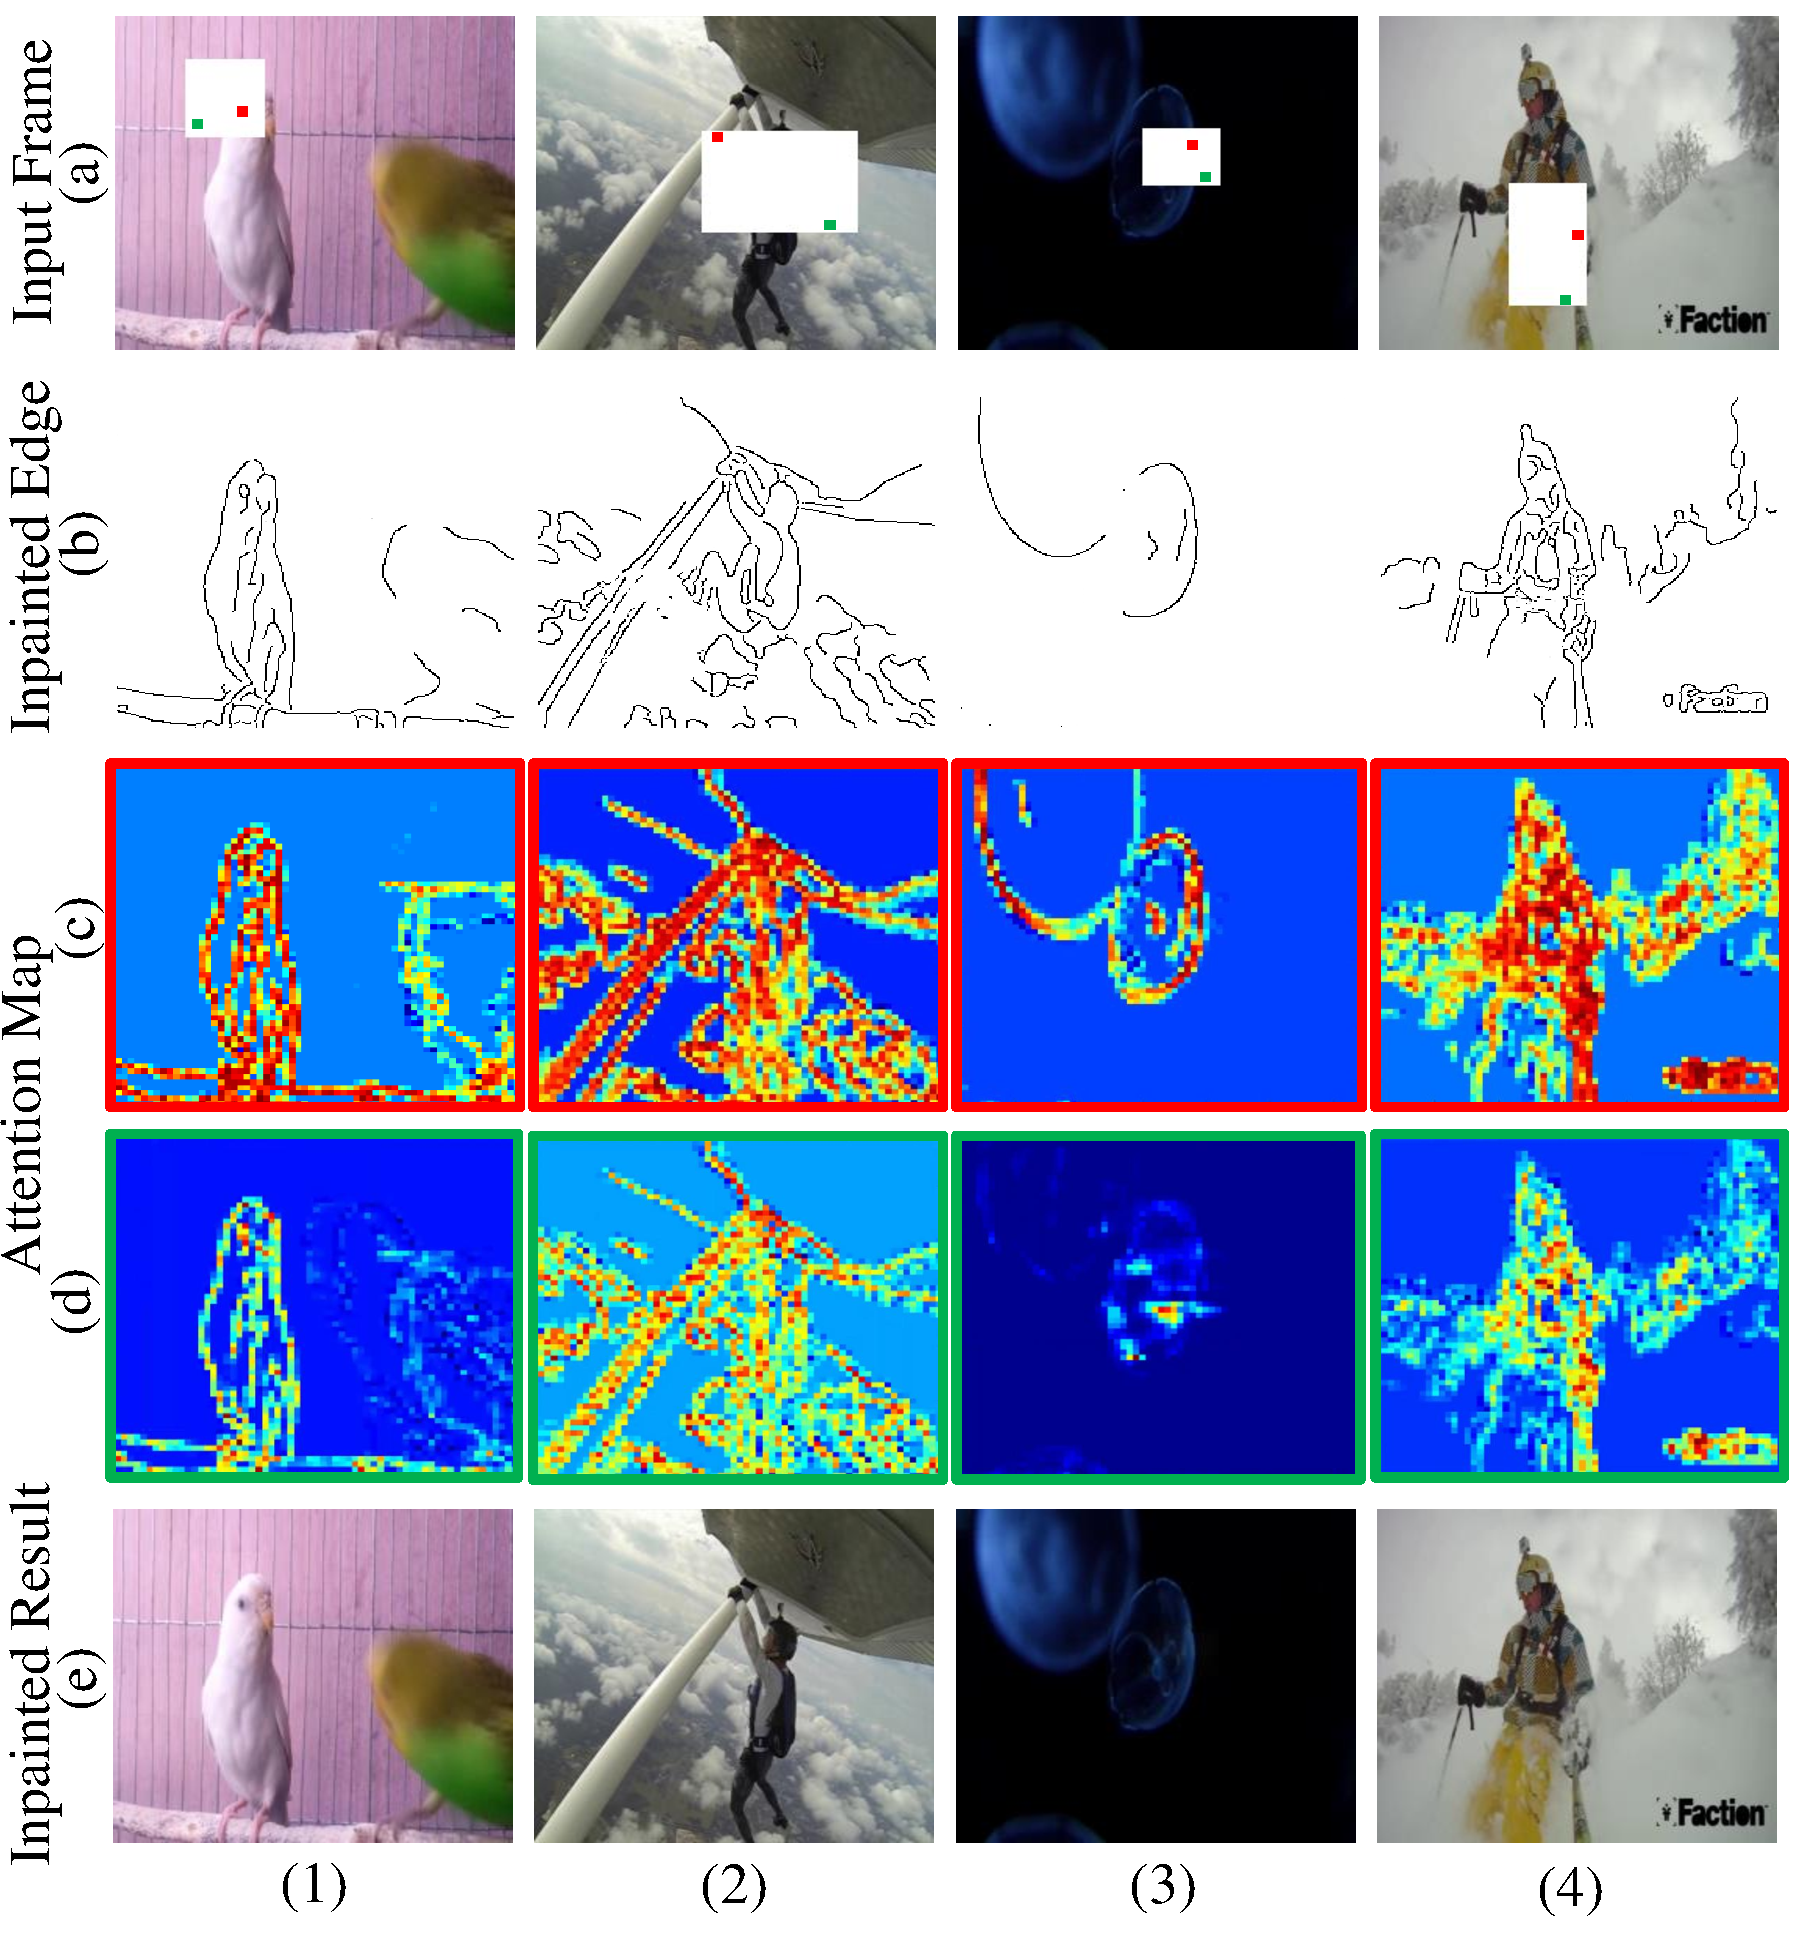
\includegraphics[width=1.0\columnwidth]{att} % Reduce the figure size so that it is slightly narrower than the column. Don't use precise values for figure width.This setup will avoid overfull boxes. 
	\caption{Visualization of attention maps in the proposed SAM. 	
	(a) A foreground pixel (red) and a background pixel (green) in a corrupted frame. (b) The completed edge maps by ENet. (c) and (d)
	The attention maps show the correlations between the selected foreground/background pixels and other regions respectively. (e) The final inpainting results from the refinement network with structural guidance. }
	\label{fig:att}
\end{figure}





\subsubsection{Visualization of Structure Attention}

To further reveal the effect of our proposed structure attention module (SAM) in the TexNet, we visualize the attention maps produced during the inpainting process for a group of examples in Fig.~\ref{fig:att}.
For each example, we pick a foreground pixel (red) and a background pixel (green) in the missing region, and show their corresponding attention maps.
%
While the coarse inpainting network in TexNet effectively produces most low-frequency signals in the missing regions, the refinement network aims to add high-frequency signals such as visual details and sharp edges for both foreground and background pixels.
%
As shown in Fig.~\ref{fig:att} (c) and (d), most of these high-frequency information comes from the edge pixels.
%
Especially, in terms of the foreground pixels, the attention maps show that the refinement network aggregates information mainly from the edge pixels to preserve a consistent and clear object shape, which makes the results visually reasonable, as Fig.~\ref{fig:att} (c) shows.
In comparison, to complete the background pixels, the SAM adaptively collects information from different regions with relatively lower correlation with the edge pixels, as shown in Fig.~\ref{fig:att} (d).
%
In the first and third examples, SAM derives small weights for those edge regions to complete the background pixels with smooth textures. 
For the background pixels in the second and fourth examples, high-frequency information is necessary, where the SAM derives higher weights for edge pixels in the attention maps.  
%
The visualization shows that the proposed SAM exploits information from the edge pixels for the refinement network, which is effective in embedding the structural guidance into high-quality texture generation.



{\color{blue}
\subsubsection{Different Architectures of ENet}
We adopt a hybrid 3D+2D convolution architecture for ENet. To justify such a design, we compare our hybrid 3D+2D architecture with two variants: 1) Variant-1: directly replacing the 2D convolutions of ENet with 3D convolutions, which has the same layer numbers with our hybrid 3D+2D architecture; and 2) Variant-2: replacing the 2D part with fewer 3D convolution layers while keeping similar number of network parameters with our current architecture. The results are shown in Table \ref{tab:com-enet-arch}. It can be seen that the performance of Variant-1 is slightly better than ours, because 3D convolutions can capture finer temporal details and introduce spatial information from features of neighbor frames. However, it takes $\sim2.5\times$ parameter numbers over our hybrid 3D+2D architecture, which is a huge burden. Variant-2 results in lower generation quality because of its shallower intermediate layers. 
In comparison, our hybrid 3D+2D convolutions architecture can achieve comparable results with Variant-1 but much fewer parameters, demonstrating its better balance between computational cost and inpainting quality.

}

\begin{table}[t]
	\caption{Comparison of different architectures of ENet. }\smallskip
	\scriptsize
	\centering
	{
		\smallskip\begin{tabular}{c|c|c|c|c}
			\hline
			&\multicolumn{3}{c|}{Free-Form Mask}& \#Params of ENet \\
			\cline{2-4} 
			& PSNR & SSIM & FID  & (M) \\
			
			\hline
			Variant-1  &\textbf{35.8167} &\textbf{0.9714} & \textbf{3.8173}& 32.29 \\ \hline
			Variant-2 & 34.9607& 0.9667& 5.9657& 14.59
			\\ \hline
			Ours
			&\underline{35.7783}  &\underline{0.9712}  &   \underline{5.8786}  & 13.41 \\
			\hline
			
			
		\end{tabular}
	}
	\label{tab:com-enet-arch}
\end{table}

\begin{figure}[t]
	\centering
	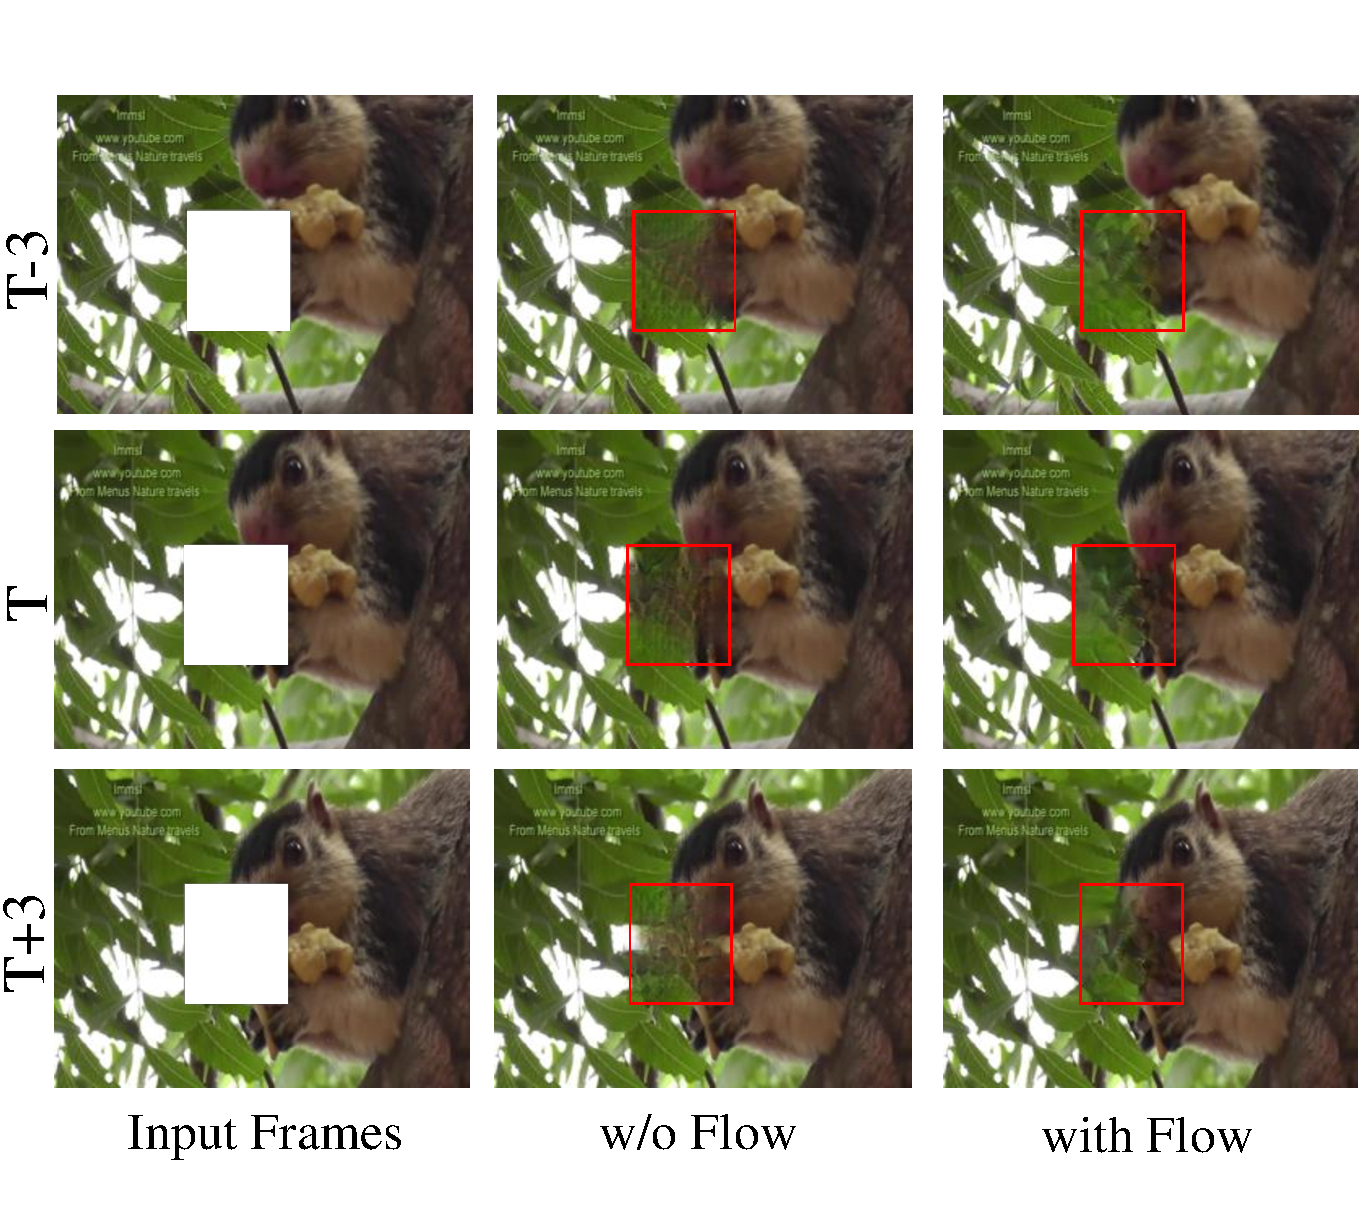
\includegraphics[width=0.9\columnwidth]{flow_vis} % Reduce the figure size so that it is slightly narrower than the column. Don't use precise values for figure width.This setup will avoid overfull boxes. 
	\caption{Inpainting results of three neighboring frames. With the flow constraints during network training, the inpainting results are more temporally consistent without introducing image blurs. }
	\label{flow_vis}
\end{figure}







\subsubsection{Effect of Flow for Temporal Coherence}

%Temporal coherence is an important factor in video inpainting. 
We utilize temporal information to smoothen artificial flickers via two developed flow-guided warping losses during training. 
Table~\ref{tab:abl} shows that the quantitative performance is improved on all three mask settings by adding the flow guidance. 
{\color{blue}According to the metric of Tem-ERR, our results are temporally smoother when the generation quality improves as gradually adding edge and SAM. Adding the guidance of optical flow brings huge enhancement to temporal consistency. %This demonstrates the effect of flow guidance.
}
Especially, we only add flow guidance in the training phase. 
Thus it brings performance gains without extra computation costs during testing.
%However, the performance improvement brought by the flow constraints is smaller than the gain caused by structural guidance.The reason is that the flow is only used in the training stage as temporal guidance, while the edge is used during the inference.
%It should be noted that predicting the completed optical flow among several frames takes more time than the edges during inference.
%Thus, we use the flow in training and the structure edge in both training and testing, which can achieve a good balance between the quality improvement and the inference efficiency. 
%
As Fig.~\ref{flow_vis} shows, the synthesized contents in neighboring frames become more temporally consistent by adding the flow constrained losses.
This proves that the proposed two flow-guided constraints in edge and texture inpainting networks are effective in enhancing temporal consistency.
%and the color changes between neighboring frames become less obvious after employing flow.
%The comparison can be better illustrated in the supplementary video.
%Note that the performance gain from the temporal information is smaller than that from structure guidance in this paper.
%The reason might be that our baseline model has a certain ability to utilize complementary information from neighboring frames.

%Both the quantitative and qualitative results prove that the motion information is beneficial to temporal consistency as well as inpaitning.

\begin{figure}[t]
	\centering
	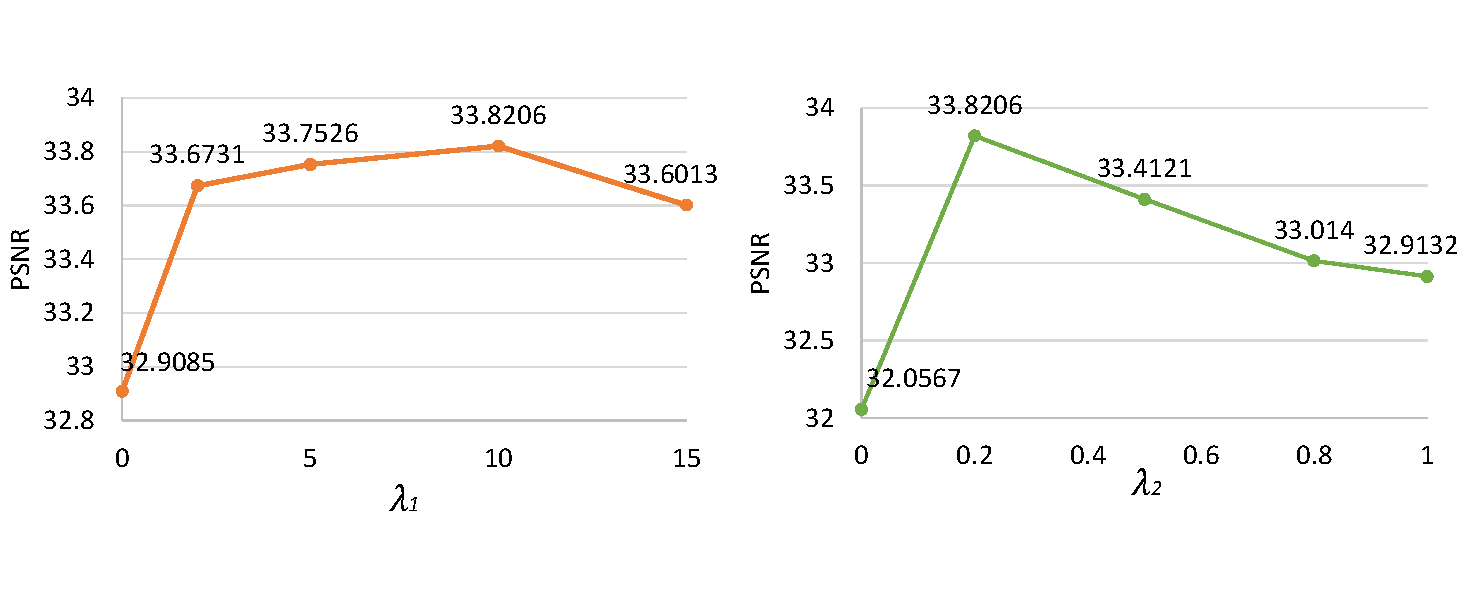
\includegraphics[width=1.0\columnwidth]{lamda1} % Reduce the figure size so that it is slightly narrower than the column. Don't use precise values for figure width.This setup will avoid overfull boxes. 
	\caption{Comparison of hyper parameters $\lambda_1$ and $\lambda_2$. The best result is obtained when $\lambda_1=10.0$ and $\lambda_2=0.2$.}
	\label{fig:hparam}
\end{figure}




 


\subsubsection{Effects of Different Hyper Parameters}
%n our experiment, we set $\lambda_1=10.0,\lambda_2=5.0$.
We conduct experiments to determine the hyper-parameters of $\lambda_1$ in Eq.~\eqref{eq:loss_e_} and $\lambda_2$ in Eq.~\eqref{eq:loss_rec}. 
We use the integration model of ENet and TexNet in this experiment without SAM and flows.
We first train ENet with different values of $\lambda_1$, and then train TexNet with recovered edge maps while fixing ENet. The value of $\lambda_2$ is set as $0.2$ when testing different $\lambda_1$.
When determining $\lambda_2$ for TexNet, we set $\lambda_1=10.0$.

$\lambda_1$ is used in Eq.~\eqref{eq:loss_e_} as a weight of feature matching loss when training ENet. %The quality of generated edge maps should be measured by the quantitative results of inpainted frames in task of video inpainting. 
%Thus, 
From the curve in Fig.~\ref{fig:hparam}, when increasing $\lambda_1$ from $0.0$ to $2.0$, the performance gain is obvious, which proves that the feature matching loss is effective in
generating high-quality edge maps used for the final inpainted results. 
Then when $\lambda_1$ is increased from $2.0$ to $10.0$, slight improvement is obtained.
The model obtains the best performance at $\lambda_1=10.0$.
%Therefore, we set $\lambda_1$ to $10.0$ for the experimental settings.
%
$\lambda_2$ in Eq.~\eqref{eq:loss_rec} is the weight of $l_1$-reconstruction loss of the coarse prediction in TexNet. 
When $\lambda_2$ is $0.0$, the TexNet is trained without the supervision of the coarse prediction, and the inpainting quality is significantly harmed.
% the result is heavily harmed. 
It demonstrates that the coarse-to-fine architecture is effective in TexNet. The best performance is obtained when $\lambda_2=0.2$. And performance drops when $\lambda_2>0.2$, which reflects that the supervision on the fine prediction networks is more important.
Therefore, we set $\lambda_2$ as $0.2$ in all the other experiments.
%Results are shown in Fig.~\ref{fig:hparam}. As shown, $\lambda_1=10.0,\lambda_2=5.0$ is the best choice.




\begin{table}[t]
	\caption{Comparison of different input frame gaps. }\smallskip
	\scriptsize
	\centering
	{
		\smallskip\begin{tabular}{c|c|c|c|c}
			\hline
			&\multicolumn{4}{c}{Free-Form Mask}  \\
			\cline{2-5} 
			Frame Gap& PSNR & SSIM & FID & Tem-ERR \\
			
			\hline
			$\{V_{t-4},V_{t-2},V_{t},V_{t+2},V_{t+4}\}$ 
			& 35.4981 & 0.9675 & 6.2889 &\textbf{0.02240} 
			\\ \hline
			$\{V_{t-15},V_{t-8},V_{t},V_{t+8},V_{t+15}\}$ & 32.2267 & 0.9505 &  10.2866 &0.02826
			\\ \hline
			Ours &\textbf{35.9613} & \textbf{0.9721}&  \textbf{5.8694} &  0.02278 \\
		
			\hline
			
			
		\end{tabular}
	}
	\label{tab:input-gap}
\end{table}

\begin{table}[t]
	\caption{Comparisons on Different sizes of holes. }\smallskip
	\scriptsize
	\centering
	\resizebox{1.0\columnwidth}{!}{
		\smallskip\begin{tabular}{c|c|c|c|c|c|c}
			\hline
			&\multicolumn{6}{c}{Fixed Square Mask} \\
			\cline{2-7}
			 Hole Size& \multicolumn{2}{c|}{$120\times120$} & \multicolumn{2}{c|}{$60\times60$} & \multicolumn{2}{c}{$30\times30$} 
			\\
			\cline{2-7}
			& PSNR & SSIM  & PSNR & SSIM  & PSNR & SSIM\\
			
			\hline
			
			
			
			Edge-Connect \cite{nazeri2019edgeconnect} & 22.6476 & \underline{0.8805} & 30.8471 & 0.9725 & 36.0358 & 0.9908\\
			\hline
			CombCN \cite{wang2019video} & 22.0341 & 0.8710 & 29.9125 & 0.9712 & 34.1423 & \underline{0.9935}\\
			\hline
			
			
			DVI \cite{Kim_2019_CVPR1}&22.1226 & 0.8693 & 28.8842 & 0.9565 & 34.5024 & 0.9780 \\
			\hline
			
			DFVI \cite{Xu_2019_CVPR} & 21.9887 & 0.8750 &  30.2409 & \underline{0.9686} & \underline{37.6599}  & 0.9920 \\
			\hline
			
			Copy-and-Paste \cite{lee2019copy}&
		22.6380 & 0.8484 &29.7965 & 0.9286 & 33.9894 & 0.9474
			\\
			
			\hline
			
			
			OPN \cite{oh2019onion} & \textbf{23.5713} & 0.8619 & \underline{31.2211} &  0.9338 & 36.9422 & 0.9694\\
			
			
			\hline
			
			
			
			
			Ours &\underline{23.2086}   &\textbf{0.8876}  & \textbf{32.5849} & \textbf{0.9763}  & \textbf{42.3711} & \textbf{0.9952}\\
			\hline
			
			
			
			
		\end{tabular}
	}
	\label{tab:holesize_com}
\end{table}




\begin{table}[t]
	\caption{Comparisons on Higher resolution. }\smallskip
	\scriptsize
	\centering
	{
			\smallskip\begin{tabular}{c|c|c|c}
			\hline
			&\multicolumn{3}{c}{Free-Form Mask} \\
			\cline{2-4} 
			& PSNR & SSIM & FID\\
			
			\hline
			
		Edge-Connect \cite{nazeri2019edgeconnect} &29.2517 &0.9373 &  24.5495\\
	\hline
	CombCN \cite{wang2019video} & 31.5213 & 0.9531 & 15.9324 \\
	\hline
	
	
	DVI \cite{Kim_2019_CVPR1}&32.3845  &0.9618 & 11.7138 \\
	\hline
	
	DFVI \cite{Xu_2019_CVPR} & 33.8953 & 0.9601 & 12.5124 \\
	\hline
	
	Copy-and-Paste \cite{lee2019copy}&
	 31.8301 &  0.9412  & 10.7987
	\\
	
	\hline
	
	
%	OPN \cite{oh2019onion} & \multicolumn{3}{c}{-} \\
	
	
%	\hline
	
	
	
	
	Ours &\textbf{36.7582} & \textbf{0.9790} &\textbf{3.7577}  \\
	\hline
		
			
		\end{tabular}
	}
	\label{tab:higherres_com}
\end{table}



{\color{blue}
	\subsubsection{Different frame gaps}
	
We conduct experiments to evaluate the effects of different frame gaps. In our default setting, we use $T$ frame $\msset{V}$ as input in our method. In this experiment, we try a small gap, $\{V_{t-4},V_{t-2},V_{t},V_{t+2},V_{t+4}\}$, and a large gap,
$\{V_{t-15},V_{t-8},V_{t},V_{t+8},V_{t+15}\}$. Results are shown in Table \ref{tab:input-gap}, which show that: a) the smaller gap will make inpainting results temporally smoother but may lose some distant frame information, and b) the larger gap will harm both spatial and temporal coherence, because it may introduce noise from long-range frames. So we finally choose a trade-off setting with gap of $\msset{V}$, which achieves a balanced performance.

}


%We also notice that the best performance is typically obtained when using moving square masks for each individual approach. It indicates that these inpainting network can learn complementary information from neighboring frames.Some inpainting examples are shown in Fig.~\ref{viszong}.Compared with existing methods, the inpainting results predicted by our method are more realistic with finer details. We can observe that the frames completed using our method contain sharper object boundaries. This is achieved by the effectiveness of structure information in video inpainting.%It can also be seen that our method produces temporally smooth results when observing neighboring frames. More comparisons can be found in thesupplementary video. %\cxj{show results?}
\subsubsection{Generalization to  Different Hole Size}
{\color{blue}	To investigate the stability of our method on different hole sizes, we compare the performance of experimental methods on three hole settings, of which the results are listed in Table \ref{tab:holesize_com}. The experiments are conducted on corrupted images with fixed square mask setting. The three kinds of hole sizes are: 1) Large hole: $120\times120$. 2) Medium hole: $60\times60$. 3) Small hole: $30\times30$. As shown in Table \ref{tab:holesize_com}, the performance of all the methods drops heavily when testing on larger holes. Our method achieves the best performance under most circumstances, except for the PSNR under the large hole size. The PSNR under large hole size of our method is slightly worse than that of OPN, which copies useful information from other frames. However, our method is much better than OPN under other settings. The results show that the performance of our method is stable on different hole sizes.

\subsubsection{Generalization to Higher Input Resolution}
We also conduct experiments on higher resolution. We use models trained on small sizes to test on image size $1024\times512$. Results are shown in Table \ref{tab:higherres_com}. Notably, OPN is not compared, which takes too much memory cost and cannot be deployed on the GPU we use. Our method can achieve decent performance under high resolution. The results demonstrate the effectiveness of our method.
}
 

